\documentclass{article}
\usepackage{amsmath}
\usepackage{listings}
\usepackage{xcolor}
\usepackage{indentfirst}
\usepackage{pgfplots}

% Set pgfplots compatibility mode
\pgfplotsset{compat=1.18}

\title{Probabilistic Analysis and Computational Modeling of Dice Rolls in Tabletop Games}
\author{NotAShelf}

% Define code listing style
\lstdefinestyle{mystyle}{
    backgroundcolor=\color{white},
    basicstyle=\ttfamily\small,
    breakatwhitespace=false,
    breaklines=true,
    captionpos=b,
    keepspaces=true,
    numbers=left,
    numbersep=5pt,
    numberstyle=\tiny\color{gray},
    showspaces=false,
    showstringspaces=false,
    showtabs=false,
    tabsize=2
}

\lstset{style=mystyle}

\begin{document}
\maketitle

\tableofcontents

\section{Introduction}

Dice rolling is a fundamental element in the world of tabletop games, to which I have recently taken a liking to, and
understanding the probabilities associated with rolling specific numbers on a fair $n$-sided die is essential
for both game enthusiasts and mathematicians. This "paper" provides a comprehensive explanation of the
mathematical concepts that underpin the calculation of these probabilities, as well as the implementation of
these concepts in a C++ program to demonstrate the practical application of these mathematical concepts.

\subsection{Inspiration}

Believe it or not, this program was inspired by the game Baldur's Gate 3, where you are constantly required to
roll dice as per its Dungeons \& Dragons origin. The idea for the program sprung from a certain occasion
where I managed to land the dice on 19 (when I needed a 20) two times in a row, which piqued my curiosity about the
mathematical probability of such an event, and eventually lead me to write a program to calculate said possibilities.


\section{Probability of Rolling a Specific Number}

The probability of rolling a particular number, denoted as $x$, on a fair $n$-sided die can be calculated
using a simple, straightforward formula that is as follows:

\[
P(x) = \frac{1}{n}
\]

\begin{align*}
Where P(x) & \text{ is the probability of rolling the number } x. \\
n & \text{ is the number of sides on the die.}
\end{align*}

However, not all dice are fair. And unfair dice can have biased probabilities, which affect
the likelihood of specific outcomes. For instance, consider an unfair 6-sided die with the following probabilities:

\[
\begin{aligned}
P(1) & = 0.1 \\
P(2) & = 0.1 \\
P(3) & = 0.1 \\
P(4) & = 0.1 \\
P(5) & = 0.1 \\
P(6) & = 0.5 \\
\end{aligned}
\]

In this case, the probability of rolling '6' is significantly higher than the rest, making it more likely
compared to the other numbers. The graph below illustrates the compared probabilities of rolling '6' on both a fair and
an unfair 6-sided die.

\begin{center}
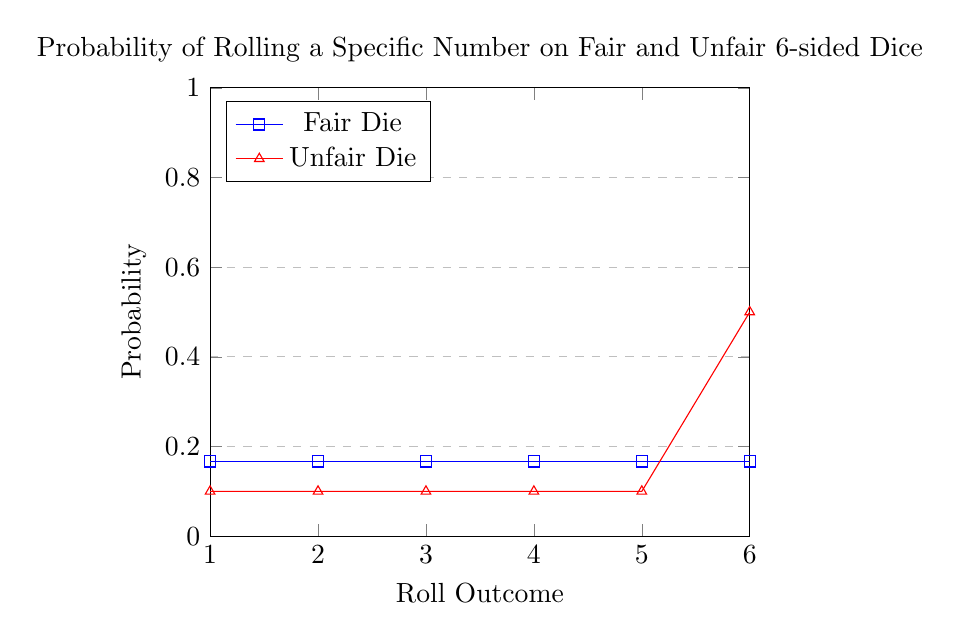
\begin{tikzpicture}
\begin{axis}[
    title={Probability of Rolling a Specific Number on Fair and Unfair 6-sided Dice},
    xlabel={Roll Outcome},
    ylabel={Probability},
    ymin=0, ymax=1,
    xmin=1, xmax=6,
    xtick={1,2,3,4,5,6},
    ytick={0,0.2,0.4,0.6,0.8,1.0},
    legend pos=north west,
    ymajorgrids=true,
    grid style=dashed,
]

\addplot[
    color=blue,
    mark=square,
    ]
    coordinates {
    (1,0.1667)(2,0.1667)(3,0.1667)(4,0.1667)(5,0.1667)(6,0.1667)
    };

\addplot[
    color=red,
    mark=triangle,
    ]
    coordinates {
    (1,0.1)(2,0.1)(3,0.1)(4,0.1)(5,0.1)(6,0.5)
    };

\legend{Fair Die, Unfair Die}
\end{axis}
\end{tikzpicture}
\end{center}


In the graph, the blue bar represents the probability of rolling a '6' on a fair 6-sided die, which is approximately
0.1667. The red bar represents the probability of rolling a '6' on an unfair 6-sided die, which is higher at 0.5. This
comparison demonstrates how the probabilities can differ for fair and unfair dice.

\subsection{Example: Rolling a Specific Number in Dungeons and Dragons}

Let's consider the popular (and highly enjoyable) tabletop game Dungeons \& Dragons (D\&D), where players use
various dice to determine the outcomes of their actions. In D\&D, a 20-sided die, commonly known as a d20, is often
used to determine the success or failure of certain actions.

For example, when a player attempts to hit an enemy with their sword, they roll a d20 and add their attack bonus.
If the total is equal to or higher than the enemy's armor class (AC), the attack is successful.

Suppose we want to calculate the probability of rolling a natural 20 on a d20 in D\&D. Since a d20 has 20 sides, the
probability can be calculated as:

\[
P(20) = \frac{1}{20} = 0.05 = 5%
\]

This means that, on average, a player has a 5\% chance of rolling a natural 20 on a d20 in D\&D.

\section{Probability Calculation in the C++ Program}

Now, let's delve into the C++ program that calculates these probabilities. Below is a portion of the code that
illustrates how the probability of a specific sequence is calculated:

\begin{lstlisting}[language=C++, caption=C++ Code for Probability Calculation]
// Function to calculate the probability of a specific sequence of rolls
double calculateSequenceProbability(int sides, const std::vector<int>& sequence) {
    double probability = 1.0;
    for (int value : sequence) {
        probability *= calculateProbability(sides, value);
    }
    return probability;
}
\end{lstlisting}

In the above code snippet, we have a function $`calculateSequenceProbability`$ that takes the number of sides on
the die and a sequence of rolls as input. It calculates the probability of the given sequence by multiplying
the individual probabilities of each roll. The `calculateProbability` function, as shown earlier, computes
the probability of rolling a specific number.

This C++ program provides a practical implementation of the mathematical concepts discussed earlier.

\section{Conclusion}

This paper has explored and briefly elaborated on the mathematical foundations and formulas governing the
probabilities of rolling specific numbers and sequences on a fair $n$-sided die as a means of documenting my own
adventure of understanding dice rolling probabilities. Understanding these principles is not only valuable for
game enthusiasts, such as myself, but also for mathematicians who appreciate the beauty of probability theory
in action - a premise which warranted the accompanying C++ program that demonstrates the practical
application of these mathematical concepts in assessing the likelihood of specific outcomes when rolling dice.

By applying mathematical concepts, such as the probability formula for rolling a specific number, we can gain
insights into the likelihood of certain outcomes in tabletop games, and through the implementation of a C++
program, we have demonstrated the practical application of these mathematical concepts. By calculating the
probabilities of specific sequences of dice rolls, players can make informed decisions and strategize their gameplay.

Decisive conclusion to this paper is that dice rolling is fun, and funny rocks that go click clack make my brain
release dopamine, and also that math is pretty cool.

\subsection{Future Research}

Further research could explore more complex scenarios, such as the probabilities of rolling multiple dice and
calculating the probabilities of specific combinations or patterns. Additionally, investigating the impact of
different dice rolling techniques or the use of weighted dice on the probabilities would provide valuable insights
into the fairness and integrity of tabletop games.

\section{References}

\begin{thebibliography}{2}
\bibitem{ross2008} Ross, S. M. (2008). A First Course in Probability (8th ed.). Pearson.
\end{thebibliography}


\end{document}
